\section{Artefact Development Approach}~\label{sec:approach}

\todo{intro para}

\subsubsection{GNU Radio block diagram}

Each radar was simulated in GNU radio according to the specifications outlined in the research methodology.
Figure \ref{fig:FMCW} shows the \ac{FMCW} radar model.
% 
\begin{figure}[ht]
    \centering
    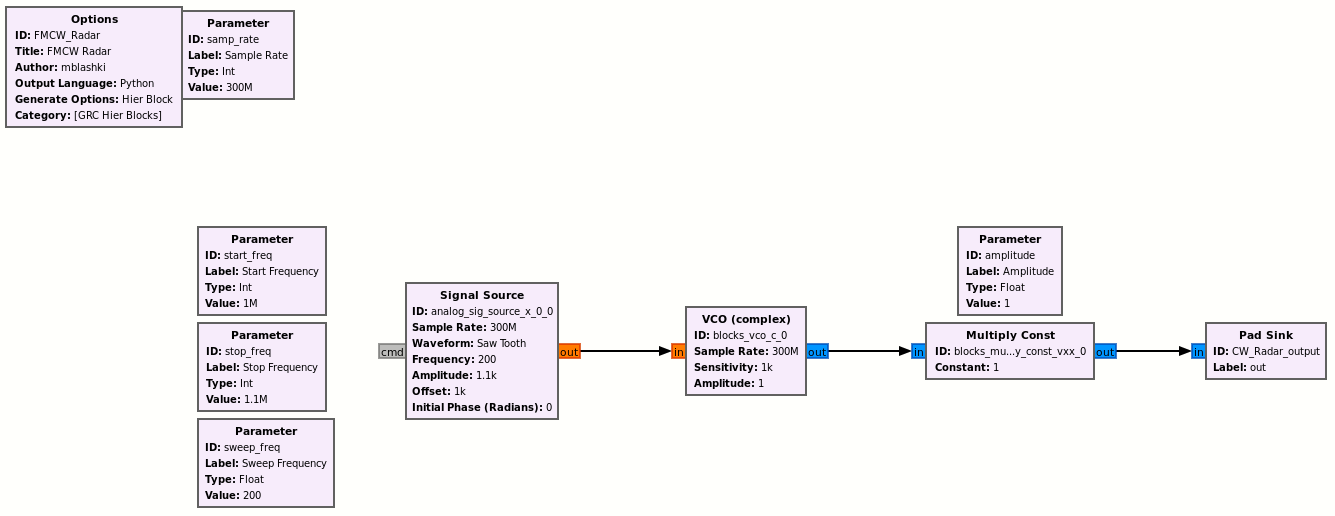
\includegraphics[width=1\textwidth]{Figures/FMCW.png}
    \caption{\ac{FMCW} radar model}
    \label{fig:FMCW}
\end{figure}
% 
Figure \ref{fig:pulsed_CW} shows the un-modulated pulsed radar model.
% 
\begin{figure}[ht]
    \centering
    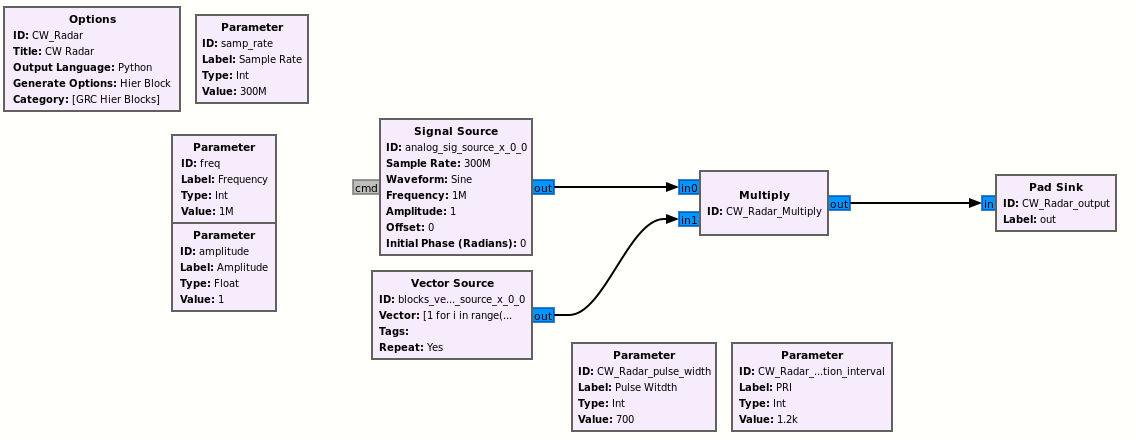
\includegraphics[width=1\textwidth]{Figures/pulsed.png}
    \caption{Pulsed \ac{CW} radar model}
    \label{fig:pulsed_CW}
\end{figure}
% 
The in-built 'Signal Source' block was used for the \ac{CW} radar model.

Figure \ref{fig:test_bed} outlines the block diagram used for experimentation.
% 
\begin{figure}[ht]
    \centering
    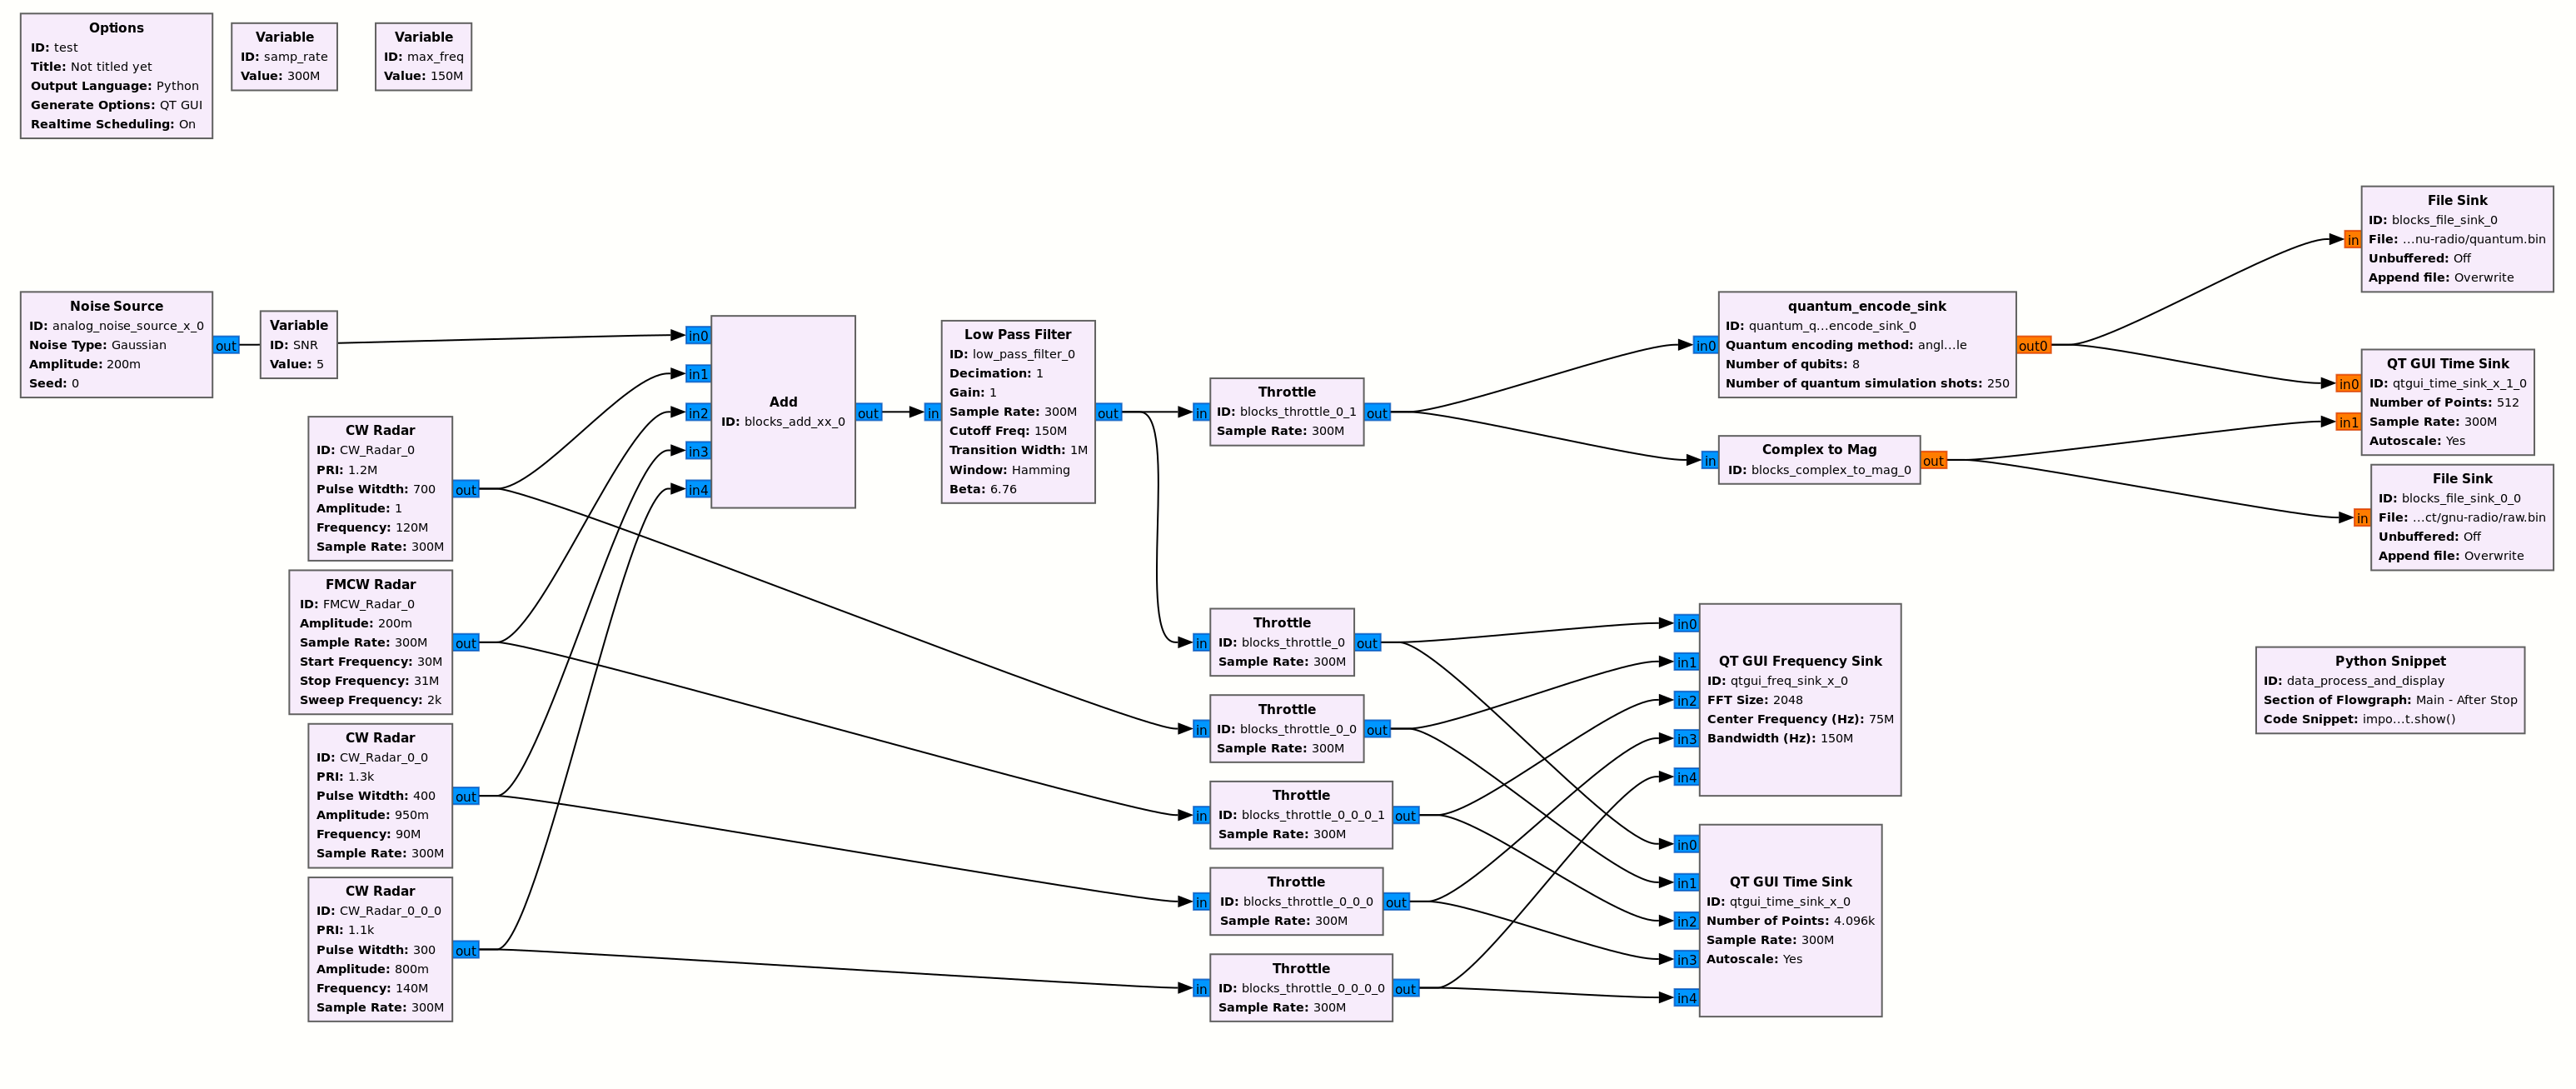
\includegraphics[width=1\textwidth]{Figures/test_bed.png}
    \caption{Test and experimentation block diagram}
    \label{fig:test_bed}
\end{figure}
Testing and experiment runs were conducted with multiple radar signals being summed together, with an added noise source.
A spectrum view and time-domain view were used for debugging.
The quantum encoding block \lstinline{quantum_encode_sink} was created that takes a \lstinline{np.complex64} data type, and outputs a \lstinline{np.float32}.
Throttles were added to ensure all signals were synchronised with the sample rate.
\lstinline{quantum_encode_sink} was parameterised with number of qubits and shots (or number of measurements to take per sample).
Figure \ref{fig:quantum_encode_sink_parameters} details the parameters used for these experiments
% 
\begin{figure}[ht]
    \centering
    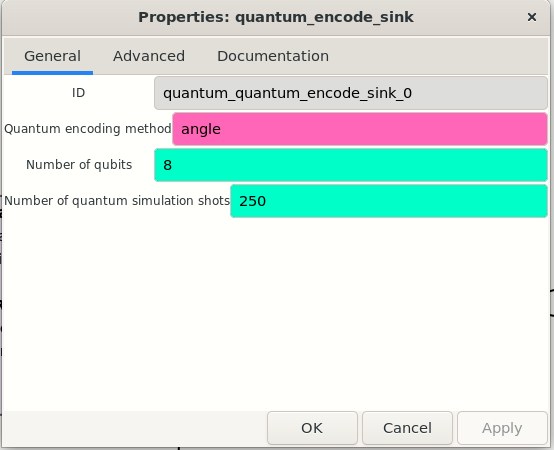
\includegraphics[width=1\textwidth]{Figures/quantum_encode_sink_parameters.png}
    \caption{\lstinline{quantum_encode_sink} parameters}
    \label{fig:quantum_encode_sink_parameters}
\end{figure}


% ---------------- EXPERIMENT 1 ---------------- %
\subsection{Experiment 1}
\todojc{We need some paragraph describing what is the aim of the subsections and what we are going to find in them.}
\todojc{Also this chapter is to include some details of the "development artefact", which are the details of your development environment, some description of your program design, some code decisions, etc.}

\textbf{Artefact}

The encoding was implemented in a single class which inherits from a GNU basic block.
It uses several libraries: logging, math, sys, Counter, matplotlib.pyplot, numpy, pywt, gnuradio, and qiskit.
In the initialisation method, it sets up logging, selects the encoding method, and configures various parameters such as the number of qubits and shots.
The class overrides the general\_work method, which is called by GNU Radio to process input and produce output.
The general\_work method retrieves the input buffer, initializes quantum and classical registers, performs the encoding based on the selected method, measures the quantum circuit, runs simulations, and retrieves the measurement results.
It has three selectable encoding options: 'basis', 'amplitude', and 'angle'.

To save the data, two file sinks were added, which act as the final output of the experimentation system. One sink saves the measured quantum data, while the other captures the raw input data

There is also an auxiliary block that completes final post-processing operations when the simulation is exited.
Specifically, it loads data from the two saved binary files (quantum.bin and raw.bin) and store them in arrays using numpy.fromfile.
It then combines them and saves it to a CSV file named data.csv.
The data are then plotted against the sample index using matplotlib.pyplot.plot, and displayed in a chart.

\textbf{Method}

The incident signal prior to sampling is a continuous complex-valued function
$x : \mathbb{R} \rightarrow \mathbb{C}, t \mapsto x(t)$,
where $x(t)$ represents the complex amplitude of the signal at any given time, $t \in \mathbb{R} > 0$.

The continuous signal is quantised,
$x : \mathbb{N} \rightarrow \mathbb{C}, t \mapsto x[t]$,
where $x[n] = x(n T_s)$, the $n^{th}$ sample of the signal, $n$ is an integer representing the sample index, and $T_s$ is the sampling period (i.e., $T_s = 1/f_s$).\footnote{$f_s$ is the sampling frequency of $300MHz$}

Let $\mathbf{x}$ be the buffer of samples $x_n=x[n]$.

The goal of encoding is to prepare the sample buffer for quantum processing.
Basis encoding, amplitude encoding, and angle encoding will be tested.

\textbf{Basis encoding}

The simplest of all non-trivial quantum encoding methods, basis encoding, maps a binary string $x \in {\{0,1\}}^n$ as coefficients of basis states.\footnote{In this paper,the convention of the computational basis is adopted, where the basis states are represented by the standard computational states $\ket{0}$ and $\ket{1}$.}

Let $\vert b_n \rangle$ be the $n^{th}$ orthonormal basis for a $N$-dimensional quantum system.
Then any state of the system can be written as a linear combination of the basis states:
\begin{equation}
    \displaystyle{
        \mathbb{R}^N \rightarrow | \mathbf{x} \rangle =
        \sum_{i=0}^{N-1}
            c_i | b_i \rangle
    }
\end{equation}
Where $c_i$ are complex coefficients of the basis states which satisfy the normalisation condition:
\begin{equation}
\label{eqn:normalisation_constraint}
    \displaystyle{\sum_{i=0}^{N-1} |c_i|^2 = \left\| \left|\psi\right\rangle \right\| = 1}
\end{equation}
% 
For basis encoding, the coefficients are further restricted such that $c_i \in \{0, k\}$, where $k \in \mathbb{R}^+$.
% 
The first step in this encoding is to define the mapping to a binary vector, $\textbf{b}$. If $\beta_i \in \{0, 1\}$ represents the $i^{th}$ bit of the transformed buffer, define $\textbf{b}$ as:
\begin{equation}
    \displaystyle{\mathbf{b} = \begin{bmatrix} \beta_0 \\ \beta_1 \\ \vdots \\ \beta_{2^{N}-1} \end{bmatrix}}
\end{equation}
% 
% Delta Encoding
% 
The transformation ($\textbf{x} \mapsto \textbf{b}$) will be a form of delta-encoding, wherein each element $d_i \in \mathbb{R}$ in array $\mathbf{D} = [d_0, d_1, \ldots, d_{2^N-1}]$ is defined by

\begin{equation}
    d_i = \lVert x[i] - x[i-1] \rVert
\end{equation}
% 
and first element defined by $d_0 = \lVert x[0] \rVert$.
% 
% Binary Encoding
% 
Given the delta array $\textbf{D}$, is real-valued and the desired transform is a binary array $\textbf{b}$, the next step proceeds to map each real element to a binary value of 1 for positive $d_i$, or 0 otherwise:
% 
\begin{equation}
    \beta_i = \begin{cases}
        1 & \text{if } d_i > 0 \\
        0 & \text{otherwise}
    \end{cases}
\end{equation}
% 
% Normalisation
% 
$\textbf{x} \mapsto \textbf{b}$, however, $\textbf{b}$ must satisfy the normalisation constraint (eqn. \ref{eqn:normalisation_constraint}).
This is done by dividing each element by the Euclidean norm, $\left\| \mathbf{b} \right\|$, yielding the normalised state vector $\left|\textbf{x}\right\rangle$.
% 
\begin{equation}
\displaystyle{
\left|\textbf{x}\right\rangle =
\frac{1}{\left\| \mathbf{b} \right\|}
\begin{bmatrix} \beta_0 \\ \beta_1 \\ \vdots \\ \beta_{2^N-1} \end{bmatrix}
}
\end{equation}
% 
Finally, the basis-encoded signal buffer is used to initialise the quantum circuit.
The implementation of which is delegated to Qiskit, using the \texttt{QuantumCircuit.initialize} method.

\textbf{Example Basis encoding}

%%%%%%%% example

% 
Given a signal buffer of four complex samples:
% 
\begin{equation}
\label{eqn:example_x_samples}
\mathbf{x} = \begin{bmatrix} 0.8 & 0.5 - 0.5j & 0.8 + 0.3j & 0.3 - 0.1j \end{bmatrix}^T
\end{equation}
% 
The magnitudes would be
% 
\begin{equation}
\mathbf{\lVert \textbf{x} \rVert} = \begin{bmatrix} 0.8 & 0.707 & 0.854 & 0.316 \end{bmatrix}^T
\end{equation}
% 
The delta array would be
% 
\begin{equation}
\mathbf{D} = \begin{bmatrix} 0.8 & -0.093 & 0.147 & -0.538 \end{bmatrix}^T
\end{equation}
% 
then, after binary decimation
% 
\begin{equation}
\mathbf{b} = \begin{bmatrix} 1 & 0 & 1 & 0 \end{bmatrix}^T
\end{equation}
% 
then normalising
% 
\begin{equation}
\ket{\mathbf{x}} = \frac{1}{\sqrt{2}}\begin{bmatrix} 1 & 0 & 1 & 0 \end{bmatrix}^T
\end{equation}
The state would then be used to initialise a quantum circuit using Qiskit, 
\texttt{circuit.initialize(np.array(list(0.707, 0, 0.707, 0)), 2)}.
% 
The circuit would be
\[
\Qcircuit {
   & \lstick{\ket{0}} & {/} \qw & \gate{\phi(\textbf{x})} & \qw & \lstick{\ket{\textbf{x}}} & {/} \qw & \meter & \cw \\
   \gategroup{1}{4}{1}{4}{.7em}{--}
}
\]
% 
where $\phi$ is the Qiskit state encoding. The measurement of this example would look like:
% 
\begin{equation}
    \bra{\textbf{x}} = \ket{\textbf{x}}^\dagger = \begin{bmatrix}  \frac{1}{\sqrt{2}} & 0 &  \frac{1}{\sqrt{2}} & 0 \end{bmatrix}
\end{equation}

\textbf{Amplitude encoding}

Amplitude encoding, similar to basis encoding, seeks to encode $\textbf{x}$ into coefficients of basis states.
However, the constraint of $c_i \in \{0, k\}$ is substituted by $c_i \in \mathbb{R}$, and therefore the binary delta transformation is extraneous.
As always, the normalisation constraint (eqn. \ref{eqn:normalisation_constraint}) must be upheld.
% 
The encoding is then simply a normalisation of the buffer:
% 
\begin{equation}
\displaystyle{
\ket{\mathbf{x}} =
\frac{1}{\left\| \mathbf{x} \right\|}
\begin{bmatrix} x_0 \\ x_1 \\ \vdots \\ x_{2^N-1} \end{bmatrix}
}
\end{equation}

\textbf{Example amplitude encoding}

Using the same sample $\textbf{x}$ as in eqn. \ref{eqn:example_x_samples}, the amplitude-encoded state vector would be
% 
\begin{equation}
\mathbf{\ket{\textbf{x}}} = \frac{\textbf{x}}{\lVert \textbf{x} \rVert} =
\begin{bmatrix} 0.570 \\ 0.356 -0.356j \\ 0.570 +0.213j \\ 0.213 -0.071j \end{bmatrix}
\end{equation}
%
The circuit would identical to that of the basis encoding, but with the differently-encoded $\ket{\textbf{x}}$:

\[
\Qcircuit {
   & \lstick{\ket{0}} & {/} \qw & \gate{\phi(\textbf{x})} & \qw & \lstick{\ket{\textbf{x}}} & {/} \qw & \meter & \cw \\
   \gategroup{1}{4}{1}{4}{.7em}{--}
}
\]
% 
The measurement would be:
% 
\begin{equation}
\bra{\textbf{x}} = \ket{\textbf{x}}^\dagger =  \begin{bmatrix} 0.8 \\ 0.707 \\ 0.854 \\ 0.316 \end{bmatrix}
\end{equation}

\textbf{Angle encoding}

Angle encoding is a method which transforms the basis state $\ket{0}^{\otimes N}$ by rotating each qubit by two orthogonal angles, $\theta$ and $\phi$.

The two angles are computed by taking a single-level discrete wavelet transform ($\psi(\textbf{x}) \mapsto ([a_0, a_1, \dots], [d_0, d_1, \dots])$) of the input sample buffer, $\textbf{x}$.
$\theta_i$ is calculated from the $i^{th}$ approximation coefficient ($a_i$) and $\phi_i$ from the $i^{th}$ detail coefficient ($d_i$).

Each $a_i$ and $d_i$ are frequency-amplitudes, so to ensure a meaningful rotation, they must be normalised $\textbf{a}, \textbf{d}: \mathbb{R}^{2^N-1} \mapsto [0, \pi]^{2^N-1}$.
Since the number of qubits, $N$, is less than the length of the approximate and detail coefficient vectors, the $N$ most-recent coefficients are encoded into $\theta_0, \dots, \theta_N$ and $\phi_0, \dots, \phi_N$.

The rotation operation can be described using the formalism of quantum gates and unitary operators.
% 
The quantum gate that performs this rotation is called a general single-qubit rotation gate or a $R$ gate, which may be represented by a $2\times2$ unitary matrix:
% 
\begin{equation}
R(\theta, \phi) = 
\begin{bmatrix}
\cos(\frac{\theta}{2}) & -e^{i\phi}\sin(\frac{\theta}{2}) \\
e^{i\phi}\sin(\frac{\theta}{2}) & e^{i\phi}\cos(\frac{\theta}{2})
\end{bmatrix}
\end{equation}
% 
$\theta$ being the angle of rotation about the X-Y plane, and $\phi$ the angle of rotation about the Z-axis.
% 
The gate is be applied to each qubit $\ket{x_i}$, with the resulting state after the rotation being obtained by:
% 
\begin{equation}
\ket{x_i^\prime} = R(\theta, \phi) \ket{x_i}
\end{equation}
% 
The resultant circuit schematic is thus:
\[
\Qcircuit {
   & & & \mbox{} & & \\
   & \lstick{\ket{0}} & {/} \qw & \gate{R(\phi_i,\theta_i)} & \qw & \lstick{\ket{\textbf{x}}} & {/} \qw & \meter & \cw \\
   & & & \dstick{\psi(\textbf{x})} \cwx[-1] &
   \gategroup{2}{4}{3}{4}{.7em}{--}
}
\]



% --------------
%%% Qualitative stuff / post hoc evals
% For although subsequent experimental trials and post hoc evaluation of the encoding methods remain as important means of assessing its suitability to the broader question, each experiment is designed to be independent of the results of the previous.
% In other words, while the success of the subsequent analyses hinges only somewhat on the quantitative comparison of encoding methods, it is the understanding of <...>. 
% Is is empirical trial and post hoc evaluation that measure this. 

% The method consists of creating a GNU-Radio block that permits the input of complex-valued samples into a buffer. The processing of samples is then done in Python and Qiskit within that block, and finally, outputted to a buffer where it is recorded.


\subsection{Experiments 2 & 3}

The stages in the of development the subsequent two artefacts are:
\begin{quote}
    \textit{
        \begin{enumerate}
            \item Encode the input data into the state of a set of qubits.
            \item Bring the qubits into superposition over many states (i.e., use quantum superposition).
            \item Apply an algorithm (or oracle) simultaneously to all the states (i.e., use quantum entanglement amongst the qubits); at the end of this step, one of these states holds the correct answer.
            \item Amplify the probability of measuring the correct state (i.e., use quantum interference).
            \item Measure one or more qubits.
        \end{enumerate}
        - Quantum computing for finance: Overview and prospects: Román Orús, Samuel Mugeld, Enrique Lizaso \todo{Add this to citations}
    }
\end{quote}

Instead of quantising signals into definite \ac{PDW}'s, the Quantum system might be able to generate a superposition of all possibilities of potential signal parameters at once.
Further processing such as pulse detection and de-interleaving may be able to be conducted at once.
This approach would investigate whether quantum methods can be used to place observed radar modes into a super-positioned and continuous state.